\setAuthor{Hans Daniel Kaimre}
\setRound{lõppvoor}
\setYear{2018}
\setNumber{G 2}
\setDifficulty{3}
\setTopic{Vedelike mehaanika}

\prob{Auk tünnis}
Suure vett täis tünni põhjas on auk, kust voolab vett välja. Graafikul on esitatud väljuva veejoa läbimõõdu sõltuvus kaugusest tünni põhjast $l$. Leidke veetaseme kõrgus tünnis.

\begin{center}
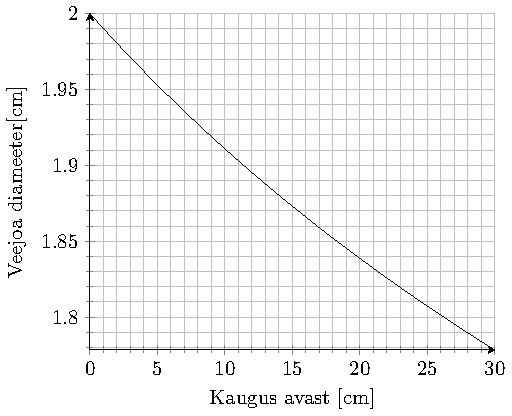
\includegraphics[width = 0.6\linewidth]{2018-v3g-02-juga.pdf}
\end{center}

\hint
Väljuva veejoa kiirus on leitav Bernoulli seadusest või energia jäävusest. Lisaks on väljuvas joas vooluhulk igas ajaühikus sama, st $Av = \const$, kus $A$ ja $v$ on vastavalt joa ristlõikepindala ja kiirus.

\solu
Veepiiril olevat vett saame vaadelda kui vedelikku vett kõrgusel $h$, mille kiirus on null ning kus rõhk peab olema võrdne õhurõhuga. Tünni põhjast väljuv juga ava juures on $h$ võrra madalamal, rõhk peab samamoodi olema võrdne õhurõhuga, kuid juga liigub kiirusega $v$. Bernoulli seadusest saame kirja panna, et $\rho g h = \rho v^2/2$, kust saame et $v^2=2gh$. Alternatiivselt saame kirja panna energia jäävuse seaduse väikese veekoguse $\Delta m$ jaoks, mille kaugus anuma põhjast on $h$: $ g h \Delta m = \Delta m \frac{v^2}{2}$, kus oleme arvestanud, et vedeliku ülemisel piiril on vee voolamiskiirus praktiliselt 0, ning et energiakadudega ei arvesta. 

Väljuvas joas peab vooluhulk ajaühikus olema sama, mis tähendab, et kehtib $A_1v_1=A_2v_2$, kus $A$ ja $v$ on vastavalt joa ristlõikepindala ja kiirus. Kuna $A=\pi d^2/4$, saame seose ümber kirjutada kujule $v_2=(d_1^2/d_2^2)v_1$. Raskuskiirendusega liikuva keha läbitud teepikkus alg- ja lõppkiiruste kaudu avaldub kui:
$$l=\frac{v_2^2-v_1^2}{2g} \Rightarrow l=\frac{\frac{d_1^4}{d_2^4}v_1^2-v_1^2}{2g} \Rightarrow v_1^2=\frac{2gl}{\frac{d_1^4}{d_2^4}-1}.$$

Vaatleme juhtu, kus $v_1=v$ on kiirus kohe ava juures. Sel juhul saame kaks avaldist $v^2$ jaoks võrduma panna:
$$2gh=\frac{2gl}{\frac{d_1^4}{d_2^4}-1}\Rightarrow h=\frac{l}{\frac{d_1^4}{d_2^4}-1}.$$

Veejoa läbimõõdu ava juures leiame graafikult punktist $l=0$, teise punkti valime ise suvaliselt: Valides selleks (28,\num{1.79}), saame vastuseks $h=28/(2^4/\num{1.79}^4-1)=\SI{50}{\cm}$.

\probeng{Hole in a barrel}
A big barrel filled with water has a hole in the bottom and the water is flowing out of it. The ratio between the diameter of the exiting water flow and the distance $l$ from the bottom of the barrel is shown in the figure. Find the height of the water level inside the barrel.
\begin{center}
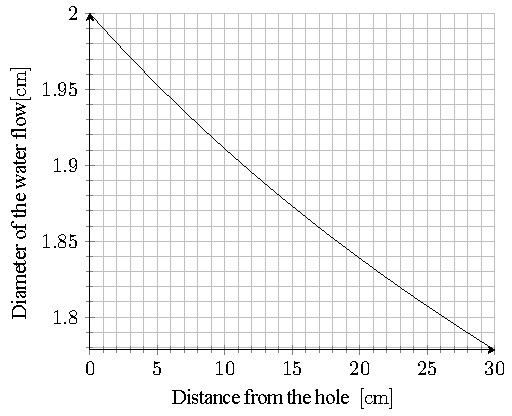
\includegraphics[width = 0.6\linewidth]{2018-v3g-02-juga_ing}
\end{center}

\hinteng
The speed of the exiting water flow can be found from the Bernoulli’s principle or the conservation of energy. In addition, the flow rate in the exiting water flow is the same for each unit of time, meaning $Av = \const$ where $A$ and $v$ are respectively the cross-sectional are and the speed of the water flow.

\solueng
The liquid at the surface of the water can be treated as being at height $h$ and flowing with a zero velocity, the pressure there is equal to the air pressure. The spurt of water exiting the barrel from the hole is lower by the height $h$, the pressure again has to be equal to the air pressure but the spurt moves with a velocity $v$. From the Bernoulli’s principle we can write down that $\rho g h = \rho v^2/2$ where we get that $v^2=2gh$. Alternatively we can write down the conservation of energy for a small amount of water $\Delta m$ which is at the distance $h$ from the bottom of the barrel: $ g h \Delta m = \Delta m \frac{v^2}{2}$, where we have taken into account that at the surface of the liquid the speed of the flowing water is practically zero and we do not consider the energy losses.\\
In the exiting spurt the flow rate has to be the same per unit of time which means that $A_1v_1=A_2v_2$ applies where $A$ and $v$ are respectively the spurt’s cross-sectional area and velocity. Because $A=\pi d^2/4$ we can rewrite the relation as $v_2=(d_1^2/d_2^2)v_1$. The distance covered by a body moving with a gravitational acceleration can expressed with initial and final velocities as:
$$l=\frac{v_2^2-v_1^2}{2g} \Rightarrow l=\frac{\frac{d_1^4}{d_2^4}v_1^2-v_1^2}{2g} \Rightarrow v_1^2=\frac{2gl}{\frac{d_1^4}{d_2^4}-1}.$$
Let us look at the case where $v_1=v$ is the velocity right at the hole. In this case we can equate two expressions for $v^2$ 
$$2gh=\frac{2gl}{\frac{d_1^4}{d_2^4}-1}\Rightarrow h=\frac{l}{\frac{d_1^4}{d_2^4}-1}.$$
We find the spurt’s diameter at the hole from the graph at the point $l=0$, the second point we choose randomly: choosing it to be (28,\num{1.79}) we get an answer $h=28/(2^4/\num{1.79}^4-1)=\SI{50}{\cm}$.
\probend